\begin{figure}[!htb]
  \centering
  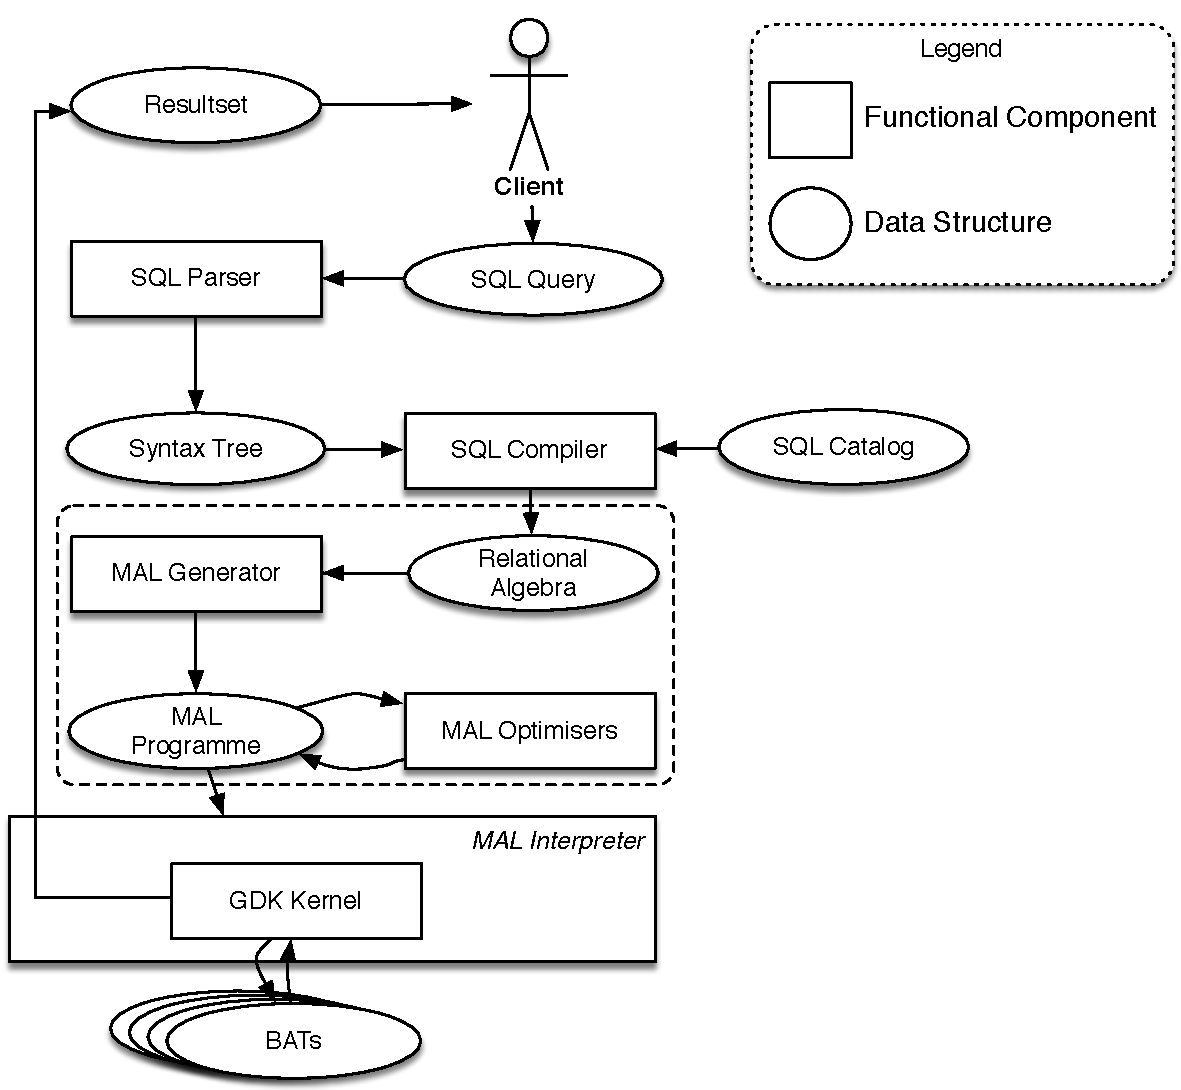
\includegraphics[width=0.9\columnwidth]{figs/MDB_architecture.pdf}
  \caption{MonetDB implementation architecture}
  \label{fig:mdbarch}
\end{figure}

\section{MonetDB Query Execution Model}
In this section we describe how the MonetDB query execution engine was used
 to develop a novel .... We also illustrate the data at our disposal to predict

\subsection{Architecture}
Figure \ref{fig:mdbarch} illustrates the components our reference system, MonetDB,
to execute an sql query. The SQL Parser and MAL Optimisers deploy well-known
rewriting rules to reduce the intermediate sizes and processing time.
It does not rely on any cost-model or pre-computed statistics
(aside from the whereabouts of the data partitions on separate nodes)

The middle layer (in the dashed box) is a sequence of specialized optimizers that morph the logical
plan received from the SQL compiler into a physical execution plan.
Constant expressions are evaluated, common sub-expressions are identified,
the dataflow graph for parallel processing is derived, etc.

The bottom layer (under the dashed box) contains the implementation of the relational operators.
Each operator takes as input the resident intermediates produced before
or accessing the persistent data on disk.
The actual implementation is often quite complex,
because each operator can be implemented in a multitude of ways.
Since the operator has full knowledge on the actual parameters,
it becomes easy to select the proper path.
Some operators even perform a sampling step before making a choice on the
 preferred algorithm.

To illustrate consider the following simple SQL query
The actual code executed by the MonetDB kernel is shown in Figure \ref{label}.
%clarify what you see

The details of the actual execution can be gathered using the Stethoscope.
A single record is shown in Figure \ref{}. Of interest to this paper are
the properties shown for the arguments and return variables.

\subsection{Profiling Information}
The MonetDB kernel can be instructed to emit profiling events.
Every primitive function comes with an event record taken at the start and
upon completion of the operation. The event record contains details on the
arguments passed, their type and size. Where ever possible the arguments
are linked with the underlying persistent column. Intermediate columns are
nameless and we only can rely on their type/cardinality.
Upon completion, we also know the exact size of the result and the time consumption.
Thread affinity is also available, but for the remainder of this paper ignored.

Explain a MAL instruction
For the remainder of this paper it is necessary to have a basic knowledge of the
MAL programming language in which all SQL queries are translated.
The MAL language is purely designed as intermediate language to express the operations.

The general format is
\begin{verbatim}
content...
\end{verbatim}
Every function belongs to a module. The arguments are either typed scalar
values (:type) or a reference to a column (:bat[:type]).
